\documentclass[conference]{IEEEtran}
\IEEEoverridecommandlockouts
% The preceding line is only needed to identify funding in the first footnote. If that is unneeded, please comment it out.
\usepackage{cite}
\usepackage{amsmath,amssymb,amsfonts}
\usepackage{algorithmic}
\usepackage{graphicx}
\usepackage{textcomp}
\usepackage{xcolor}
\def\BibTeX{{\rm B\kern-.05em{\sc i\kern-.025em b}\kern-.08em
    T\kern-.1667em\lower.7ex\hbox{E}\kern-.125emX}}
\begin{document}

\title{Project \#15: Twitter hate speech detection 2\\
% {\footnotesize \textsuperscript{*}Note: Sub-titles are not captured in Xplore and
% should not be used}
% \thanks{Identify applicable funding agency here. If none, delete this.}
}

\author{\IEEEauthorblockN{Janne Eskola}
% \IEEEauthorblockA{\textit{dept. name of organization (of Aff.)} \\
% \textit{name of organization (of Aff.)}\\
% City, Country \\
% email address or ORCID}
\and
\IEEEauthorblockN{Teemu Ikävalko}
% \IEEEauthorblockA{\textit{dept. name of organization (of Aff.)} \\
% \textit{name of organization (of Aff.)}\\
% City, Country \\
% email address or ORCID}
\and
\IEEEauthorblockN{Toni Kuosmanen}
% \IEEEauthorblockA{\textit{dept. name of organization (of Aff.)} \\
% \textit{name of organization (of Aff.)}\\
% City, Country \\
% email address or ORCID}
\and
\IEEEauthorblockN{Tapio Kursula}
% \IEEEauthorblockA{\textit{dept. name of organization (of Aff.)} \\
% \textit{name of organization (of Aff.)}\\
% City, Country \\
% email address or ORCID}
}

\maketitle

\begin{abstract}
Abstract
\end{abstract}

\begin{IEEEkeywords}
natural language processing, sentiment analysis, hate speech
\end{IEEEkeywords}
\section{Introduction}
The Cambridge dictionary defines hate speech as:
\vspace{12pt}
\emph{``public speech that expresses hate or encourages violence towards a person or group based on something
such as race, religion, sex, or sexual orientation''} \cite{Cambridge:hate_speech}
\vspace{12pt}

In practice, defining clear boundaries between hate speech and normal expression can be
hard. Legal definitions of hate speech vary by country with some countries setting much
stricter definitions of hate speech. \cite{Wikipedia:hate_speech_laws}

It could be argued that today, the largest platforms for public speech are provided by 
the social media companies, such as Facebook or Twitter. Both these companies forbid 
hate speech on their platforms \cite{Twitter:hate_speech,Facebook:hate_speech} but the sheer volume 
of posted content makes it hard to enforce these rules. The services rely on users reporting
hateful content when it is found on the platform. Facebook has also utilized machine learning
algorithms in detecting hate speech but the results have not been optimal. \cite{Time:facebook_hate_speech_languages}

Hate speech can be spread by individuals or extremist groups seeking to advance their 
agendas. Hate speech is usually directed at minorities with the aim of demonizing and 
dehumanizing the targeted group. The effects of hate speech can be severe. For example, the 
UN fact finding mission sent to Myanmar, after the government crackdown on the Rohingya 
minority, found that hate speech spread on Facebook contributed significantly to sparking 
tensions in the region\cite{Reuters:myanmar_rohingya}.

The goal of our project is to find efficient methods for identifying hate speech in online forums.
Specifically, we will target the Twitter platform. We will use the Twitter search API to retrieve and then 
manually label a hate speech data set. By examining this data set, we aim to find a potential set of features 
that could be used to identify hate speech content.  We will also profile individual posters who actively spread 
hate speech on Twitter.

\section{Problem description}
Our investigation consists of two parts. In the first part we will collect a tweet data set by searching 
for tweets with specific hashtags. This data set will be manually labeled as either hate or 
non-hate speech. We will then characterize the tweets in both categories using following features:

\begin{itemize}
    \item Sentiment analysis
    \item LIWC features
    \item Emoticon usage
    \item Named entity usage
\end{itemize}

For the second part we will identify three active twitter accounts that frequently post 
hate speech content. We will analyze the posting history of these users and calculate a 
radicalization score for each user. 

\section{Data sets}
\subsection{Data set 1: Labeled hate speech}
The first data set was collected using five specific hashtags, given to us in the assignment,
that were likely targets for hate speech. The hashtags were the following: 
\begin{itemize}
    \item \#bombing
    \item \#extremist
    \item \#islamophobia
    \item \#radicalist
    \item \#terrorist    
\end{itemize}

The tweets were collected using the Twitter premium search API with 30 day history. Retweets 
and tweets not written in English were excluded from the search. Our goal was to retrieve at least 
200 tweets per hashtag but we set the upper limit at 500. The tweets were saved as JSON files. 
After the tweets were retrieved through the API, they were labeled manually. The labels were appended  
to the original JSON schema so that all information could be preserved. 
A summary of the labeled data set is shown in table 
\ref{tab:data_set_1_summary}.

\begin{table}[!ht]
    % Add some padding to the table cells:
    \def\arraystretch{1.2}%
    \begin{center}
      \caption{Data set 1 summary}
      \label{tab:data_set_1_summary}
      \begin{tabular}{l c c c}
        \hline
        &\multicolumn{3}{c}{\textbf{Number of tweets}} \\
        \textbf{\textit{Hashtag}}& \textbf{\textit{Non-hate speech}}& \textbf{\textit{Hate speech}} & \textbf{\textit{Total}}  \\
        \cline{2-4} 
        \hline
        \#bombing & 195 & 2 & 197\\
        \#extremist & 368 & 6 & 374\\
        \#islamophobia & 158 & 12 & 170\\
        \#radicalist & 13 & 0 & 13\\
        \#terrorist & 334 & 117 & 451\\
        \hline
        \textbf{TOTAL} & \textbf{1068} & \textbf{137} & \textbf{1205}\\
        \hline
      \end{tabular}  
    \end{center}
  \end{table}

As can be seen from the table, some topics yielded very few tweets we would label as hate speech 
while some of the hashtags, especially \#radicalist, were barely used at all. We found the largest
proportion of hate speech with the terrorist hashtag (Fig \ref{fig:data_set_1_summary}). The final 
data set contained a total of 1205 tweets out of which 137 were labeled as hate speech. 

\begin{figure}[htbp]
\centering
\centerline{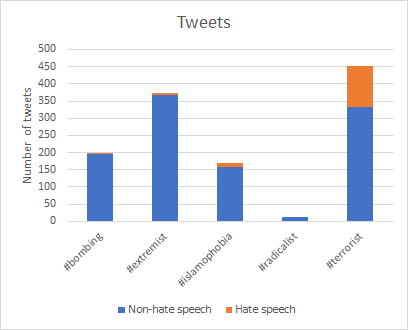
\includegraphics[width=2.5in]{data_set_1_summary.png}}
\caption{Hate/non-hate tweets per each hashtag.}
\label{fig:data_set_1_summary}
\end{figure}

\subsection{Data set 2: Active hate speakers}
For the second data set, we looked for active twitter users who frequently posted hate speech content. 
The search was limited to English speaking users only. In the end, we chose three users who fit our 
criteria: 
\begin{itemize}
    \item User 1: An UK citizen and a blogger frequently posting hate speech targeted at muslims.
    \item User 2: Active Finnish user frequently posting racist content.
    \item User 3: A former leader of an American white supremacist group.
\end{itemize}
After selecting the users, we used Twitters full archive API to retrieve thousand tweets from each user for the
radicalization analysis. 
\section{Characterization of the labeled data set}
\subsection{Sentiment analysis}
For sentiment analysis we were tasked with plotting the percentage of polarity for both annotated hate speech post and annotated non-hate speech post.
Comparing results from two different sentiment analyzers. We chose Textblob and Vader toolkits in python for using in our analysis. Both of these tools give out sentiment score values between -1 and 1
because we had to split our post based on negative, neutral and positive we choose values as following: negative (-1 – (-0,333…)), neutral (-0,333… - 0,333…) and positive (0,333… - 1).
Analysis was performed so that every tweet that we had was cleaned so that only the text part of tweets remained, these were then split to hate speech and non-hate speech and were then imported to both sentiment analyzers and result were compared.
\subsection{LIWC features}
To identify common themes and topics in the labeled tweet data set, we 
used Empath, which is an open-source alternative to proprietary LIWC software  \cite{fast2016empath}. 
The library offers tools that can extract themes and topics from a given text.
The library comes with a default set of categories but new categories can be added by the users. 
Our analysis uses the default categories.

Before the analysis, we removed the URLs and user names from the tweets. After cleaning, we analyzed each tweet text individually using Empath and counted the frequency of extracted topics in both the hate and non-hate categories. 
These raw counts were then normalized by dividing them with the number of tweets in the category. The normalized 
scores for the twenty most common topics are presented in tables \ref{tab:liwc_features_non_hate} 
and \ref{tab:liwc_features_hate}. Bar plots of the most common topics can also be found in the appendix.

\begin{table}[!ht]
    % Add some padding to the table cells:
    \def\arraystretch{1.2}%
    \begin{center}
      \caption{Top 20 most common topics in non-hate tweets}
      \label{tab:liwc_features_non_hate}
      \begin{tabular}{l c | c c}
        \hline\hline
        % \multicolumn{2}{c}{\textbf{non-hate speech}} 
        \multicolumn{4}{c}{\textbf{Non-hate speech}}\\
        \hline
        \textbf{Topic}&\textbf{Score}&\textbf{Topic}&\textbf{Score}\\
        \hline
        negative\_emotion&0.1713&terrorism&0.0927\\
        war&0.1573&weapon&0.089\\
        fight&0.1311&positive\_emotion&0.0871\\
        speaking&0.1301&violence&0.0758\\
        crime&0.1264&power&0.074\\
        communication&0.1124&business&0.0712\\
        government&0.1105&giving&0.0693\\
        aggression&0.1105&hate&0.0684\\
        kill&0.1067&law&0.0665\\
        politics&0.0946&leader&0.0655\\
        \hline\hline
      \end{tabular}  
    \end{center}
  \end{table}

  \begin{table}[!ht]
    % Add some padding to the table cells:
    \def\arraystretch{1.2}%
    \begin{center}
      \caption{Top 20 most common topics in hate speech tweets}
      \label{tab:liwc_features_hate}
      \begin{tabular}{l c | c c}
        \hline\hline
        % \multicolumn{2}{c}{\textbf{non-hate speech}} 
        \multicolumn{4}{c}{\textbf{Hate speech}}\\
        \hline
        \textbf{Topic}&\textbf{Score}&\textbf{Topic}&\textbf{Score}\\
        \hline
        negative\_emotion&0.2847&crime&0.1168\\
        hate&0.2701&appearance&0.1168\\
        children&0.219&speaking&0.1095\\
        family&0.2117&fight&0.1095\\
        love&0.2044&government&0.1022\\
        youth&0.1898&giving&0.0949\\
        emotional&0.1752&disgust&0.0949\\
        affection&0.1752&communication&0.0949\\
        kill&0.1679&terrorism&0.0876\\
        war&0.1168&leader&0.0876\\
        \hline\hline
      \end{tabular}  
    \end{center}
  \end{table}
\subsection{Emoticon usage}
We investigated the usage of emoticons in hate and non-hate tweets by examining the types 
of emoticons used and their frequency.  Using Emojis Python library \cite{python:emojis}, we 
listed all the distinct emoticons in every tweet. The hate speech tweets contained a total of 22 tweets which contained emoticons
while the  non-hate tweets contained 154. The percentage of tweets containing emojis was 
roughly the same in the two categories, 16 \% and 14 \% in hate and non-hate categories respectively.

The most frequent emoticons are listed in tables \ref{tab:emoticons_non_hate} and \ref{tab:emoticons_hate}. 
Bar plots of the most common emoticons can also be found in the appendix.


\begin{table}[!ht]
    % Add some padding to the table cells:
    \def\arraystretch{1.2}%
    \begin{center}
      \caption{Top 20 most common emoticons in non-hate speech tweets}
      \label{tab:emoticons_non_hate}
      \begin{tabular}{l c | c c}
        \hline\hline
        % \multicolumn{2}{c}{\textbf{non-hate speech}} 
        \multicolumn{4}{c}{\textbf{Non-hate speech}}\\
        \hline
        \textbf{Emoticon}&\textbf{Frequency [\%]}&\textbf{Emoticon}&\textbf{Frequency [\%]}\\
        \hline
        :end: & 5.43\% & :pout: & 0.47\%\\
        :bell: & 5.43\% & :muscle: & 0.47\%\\
        :point\_right: & 2.81\% & :heavy\_minus\_sign: & 0.37\%\\
        :joy: & 1.03\% & :calling: & 0.37\%\\
        :point\_down: & 0.66\% & :warning: & 0.28\%\\
        :wink: & 0.56\% & \emph{:sotwe:*} & 0.28\%\\
        :fire: & 0.56\% & :smirk: & 0.28\%\\
        :us: & 0.47\% & :wave: & 0.19\%\\
        :uk: & 0.47\% & :thumbsup: & 0.19\%\\
        :rofl: & 0.47\% & :smile: & 0.19\%\\                           
        \hline
        \multicolumn{4}{l}{\emph{*:stuck\_out\_tongue\_winking\_eye:}}\\
        \hline\hline
      \end{tabular}  
    \end{center}
  \end{table}

\begin{table}[!ht]
    % Add some padding to the table cells:
    \def\arraystretch{1.2}%
    \begin{center}
      \caption{Top 20 most common emoticons in hate speech tweets}
      \label{tab:emoticons_hate}
      \begin{tabular}{l c | c c}
        \hline\hline
        % \multicolumn{2}{c}{\textbf{non-hate speech}} 
        \multicolumn{4}{c}{\textbf{Hate speech}}\\
        \hline
        \textbf{Emoticon}&\textbf{Frequency [\%]}&\textbf{Emoticon}&\textbf{Frequency [\%]}\\
        \hline
        :joy: & 5.11\% & :stop\_sign: & 0.73\%\\
        :pout: & 4.38\% & :star\_of\_david: & 0.73\%\\
        :uk: & 1.46\% & :sparkler: & 0.73\%\\
        :thumbsup: & 1.46\% & :snake: & 0.73\%\\
        :smirk: & 1.46\% & :skull\_and\_crossbones: & 0.73\%\\
        :roll\_eyes: & 1.46\% & :skull: & 0.73\%\\
        :muscle: & 1.46\% & :point\_up\_2: & 0.73\%\\
        :clap: & 1.46\% & :point\_down: & 0.73\%\\
        :blush: & 1.46\% & :pensive: & 0.73\%\\
        :v: & 0.73\% & :menorah: & 0.73\%\\                        
        \hline\hline
      \end{tabular}  
    \end{center}
\end{table}

The most common emoticons used in the hate speech, :joy: and :pout:, don't really stand out 
and are frequently used in non hate context, although both seem to be more common in our 
hate speech data set. Other emoticons in the hate speech tweets were occured only once or twice.

The two most common emoticons in the non hate speech data set were :exit: and :bell:. 
It turns out both emoticons were frequently used by opponents of Jeremy Corbyn, who 
were active during the British general election that occurred in December 2019, at 
the same time we were collection our data sets.

\subsection{Named entities}
We investigated the use of named entities and their frequency in tweets containing hate speech and not containing hate speech.  The tweets were analysed using spaCy natural language processing library for python. Using the default spacy model (en_core_web_sm) for entity recognition, we identified the 20 most used named entities in both sets of tweets (the sets being tweets containing hate speech and tweets that didn’t contain hate speech) and their frequency based on the size of the tweet set. We also plotted graphs of these entities and their frequency.

<Top 20 entities in hate tweets>

<Top 20 entities in non hate tweets>

<Graph of entities in hate tweets>

<Graph of entities in non hate tweets>

Note the high frequency of Terrorist and Islamophobia in tweets containing hate speech. Since the hashtags and the words used in them are recognized as named entities, these entities are high on the list since they were words used to collect tweet used in this study.
In tweets containing hate speech other frequent named entities are closely related to UK and their current political situation. Jeremy Corbyn, his political party and his relations with Pakistan were mentioned in many of the hate speech tweets.
The same trend of named entities can be seen in the frequent entities used in tweets that did not contain hate speech. Many of the most frequent entities are related to United Kingdom and Jeremy Corbyn. Other frequent topic that can be seen in this list is the conflict between Pakistan and India, with many of the entities related to these countries and their major religions, Hinduism and Islam.

\subsection{Named phrases}
TODO
\section{Radicalization of active hate speakers}
The second dataset consist of tweets from three user accounts on Twitter that are active hate-speech spreaders. Like in the first part, only English speaking users were examined.
We aggregate a thousand tweets per user and give each user a radicalization score based on the characteristics of their tweets.

We extract the following features from their tweets per user:
\begin{itemize}
  \item Average sentiment score percentile (\(AS\))
  \item Volume of negative posts (\(VN\))
  \item Severity of negative posts (\(SN\))
  \item Duration of negative posts (\(DN\))
\end{itemize}
We use the following formula to compute a radicalization score for each user
\[Radicalization\: score = (K /AS^3) \cdot (VN \cdot SN \cdot DN)\], where \(K = 7\)
%\caption{Radicalization score formula}


\(AS\): Sentiment is within the range [-1,1], where -1 is the most negative and 1 the most positive sentiment.
 This range must be normalized to [0,1] to be used as intended in the radicalization score formula.\\ %\ref{}
\(VN\): The proportion of the posts that had a negative sentiment.\\
\(SN\): The proportion of the posts that had a 'very negative' sentiment. If a posts standardized value is less than negative three, it was considered as 'very negative'.
Standardized value is acuired for each sentiment value using the following formula;
\(z = (X - \mu)/\sigma\), where \(X\) is the value in question, and \(\mu\) and \(\sigma\) are the mean and the standard deviation of the dataset that the value belongs to. Standardized values have a mean of \(0\) and a standard deviation of \(1\). This means that a standardized value of 3, for example, is three standard deviations away from the mean to the positive side.\\
\(DN\): The duration, in number of days, between the oldest and newest tweet with a negative sentiment. \\
\\
\subsection{Results}
We used pythons TextBlob for calculating the sentiments of each tweet and got the following results:
First user:
\begin{table}[]
  \begin{tabular}{ll}
  mean sentiment percentile:     & 0.5246912423383495 \\
  volume of negative posts:      & 0.218              \\
  volume of very negative posts: & 0.014              \\
  number of days active:         & 77                 \\
  radicalization score:          & 11.388377331838583
  \end{tabular}
\end{table}
Second user:
\begin{table}[]
  \begin{tabular}{ll}
  mean sentiment percentile:     & 0.5016298412698412 \\
  volume of negative posts:      & 0.22               \\
  volume of very negative posts: & 0.022              \\
  number of days active:         & 503                \\
  radicalization score:          & 135.00855660731082
  \end{tabular}
\end{table}
\begin{table}[]
  \begin{tabular}{ll}
  mean sentiment percentile:     & 0.5222739147067796 \\
  volume of negative posts:      & 0.279               \\
  volume of very negative posts: & 0.012              \\
  number of days active:         & 246                \\
  radicalization score:          & 40.46910414477672
  \end{tabular}
\end{table}
\subsection{Problems}
TextBlobs default sentiment analyzator uses the same implementation as the "patterns" library does, and it has a certain drawback: it only takes adjetives into account. 
This lead to most of the tweets sentiment scores to be zero.\\





\section{Results}
Considering the hashtags that were used to collect the tweets, 
it is not surprising that Empath found negative and violent topics present 
in both hate and non-hate categories. Still, there is a marked difference in 
the scores between the two categories. The topics in the non-hate speech category 
are more evenly distributed which is to be expected due to the difference in sample size.
Even taking this into account, the topic 'hate' is still much more pronounced in the hate speech 
data set.  Surprisingly, themes like 'children', 'family', 'love', and 'youth' are also some of the 
most common topics in the hate speech category. The difference between the two categories suggest 
that Empath topics might be useful for identifying hate speech content.

The most common emoticons found in the hate speech tweets are widely used and cannot be considered hateful 
without further context. Based on our data, emoticons with more specialized meanings are rarely used and 
seem poor candidates for indicators. 
Many of the hate tweets containing the emoticon :joy: were malicious and mocking. 
Detecting the misalignment between the nominal meaning of an emoticon and the actual tone of the message could 
potentially be an efficient indicator of hateful content.

Textblob results show that about 75\%  off hate speech was positive and about 78\% off non-hate speech was also positive and rest of the post divided evenly among neutral and negative.
Surprising here is that according to textblob most of our hate speech would be positive hate speech and not negative what would be the logical solution because often hate speech is considered negative.
Same is true on non-hate speech positive is to most common polarity but this is more reasonable because tweets that are not considered to be hate should be more on the positive side. 
Vader analyzer but most of our tweets in the extreme sections of the polarity so most of hate speech is negative hate and most of non-hate speech is in the positive category.
Vader analyzing was also evenly distributed so that all categories were withing 20\% of each other’s values.
Last comparison was that we checked how many percentile units the two sentiment analyzers were of each other and maximum difference was with positive hate 45\% and least different were neutral non-hate 11\%.

The most frequently used named entities in tweets studied did not differ very much between normal tweets and hate tweets. Named entities found in the tweets used were mainly of two types. First type are named entities related to current events, mainly to Brexit that is currently ongoing in United Kingdom and Jeremy Corbyn. Some of this type of entities were in tweets that were related to the current situation between Pakistan and India.
	The other type was named entities that are closely related to hate speech but not necessarily to major current events. Examples of such entities include Nazis, Islamophobia and Terrorist.
	This analysis shows that named entities are an effective way to find topics and events that generate hate speech content. However, differentiating between hate speech and not hate speech through this method is less effective since the data sets that this analysis produced are very similar.

\section{Conclusions}







% \subsection{Units}
% \begin{itemize}
% \item Use either SI (MKS) or CGS as primary units. (SI units are encouraged.) English units may be used as secondary units (in parentheses). An exception would be the use of English units as identifiers in trade, such as ``3.5-inch disk drive''.
% \item Avoid combining SI and CGS units, such as current in amperes and magnetic field in oersteds. This often leads to confusion because equations do not balance dimensionally. If you must use mixed units, clearly state the units for each quantity that you use in an equation.
% \item Do not mix complete spellings and abbreviations of units: ``Wb/m\textsuperscript{2}'' or ``webers per square meter'', not ``webers/m\textsuperscript{2}''. Spell out units when they appear in text: ``. . . a few henries'', not ``. . . a few H''.
% \item Use a zero before decimal points: ``0.25'', not ``.25''. Use ``cm\textsuperscript{3}'', not ``cc''.)
% \end{itemize}

% \subsection{Equations}
% Number equations consecutively. To make your 
% equations more compact, you may use the solidus (~/~), the exp function, or 
% appropriate exponents. Italicize Roman symbols for quantities and variables, 
% but not Greek symbols. Use a long dash rather than a hyphen for a minus 
% sign. Punctuate equations with commas or periods when they are part of a 
% sentence, as in:
% \begin{equation}
% a+b=\gamma\label{eq}
% \end{equation}

% Be sure that the 
% symbols in your equation have been defined before or immediately following 
% the equation. Use ``\eqref{eq}'', not ``Eq.~\eqref{eq}'' or ``equation \eqref{eq}'', except at 
% the beginning of a sentence: ``Equation \eqref{eq} is . . .''

% \subsection{\LaTeX-Specific Advice}

% Please use ``soft'' (e.g., \verb|\eqref{Eq}|) cross references instead
% of ``hard'' references (e.g., \verb|(1)|). That will make it possible
% to combine sections, add equations, or change the order of figures or
% citations without having to go through the file line by line.

% Please don't use the \verb|{eqnarray}| equation environment. Use
% \verb|{align}| or \verb|{IEEEeqnarray}| instead. The \verb|{eqnarray}|
% environment leaves unsightly spaces around relation symbols.

% Please note that the \verb|{subequations}| environment in {\LaTeX}
% will increment the main equation counter even when there are no
% equation numbers displayed. If you forget that, you might write an
% article in which the equation numbers skip from (17) to (20), causing
% the copy editors to wonder if you've discovered a new method of
% counting.

% {\BibTeX} does not work by magic. It doesn't get the bibliographic
% data from thin air but from .bib files. If you use {\BibTeX} to produce a
% bibliography you must send the .bib files. 

% {\LaTeX} can't read your mind. If you assign the same label to a
% subsubsection and a table, you might find that Table I has been cross
% referenced as Table IV-B3. 

% {\LaTeX} does not have precognitive abilities. If you put a
% \verb|\label| command before the command that updates the counter it's
% supposed to be using, the label will pick up the last counter to be
% cross referenced instead. In particular, a \verb|\label| command
% should not go before the caption of a figure or a table.

% Do not use \verb|\nonumber| inside the \verb|{array}| environment. It
% will not stop equation numbers inside \verb|{array}| (there won't be
% any anyway) and it might stop a wanted equation number in the
% surrounding equation.

% \subsection{Some Common Mistakes}\label{SCM}
% \begin{itemize}
% \item The word ``data'' is plural, not singular.
% \item The subscript for the permeability of vacuum $\mu_{0}$, and other common scientific constants, is zero with subscript formatting, not a lowercase letter ``o''.
% \item In American English, commas, semicolons, periods, question and exclamation marks are located within quotation marks only when a complete thought or name is cited, such as a title or full quotation. When quotation marks are used, instead of a bold or italic typeface, to highlight a word or phrase, punctuation should appear outside of the quotation marks. A parenthetical phrase or statement at the end of a sentence is punctuated outside of the closing parenthesis (like this). (A parenthetical sentence is punctuated within the parentheses.)
% \item A graph within a graph is an ``inset'', not an ``insert''. The word alternatively is preferred to the word ``alternately'' (unless you really mean something that alternates).
% \item Do not use the word ``essentially'' to mean ``approximately'' or ``effectively''.
% \item In your paper title, if the words ``that uses'' can accurately replace the word ``using'', capitalize the ``u''; if not, keep using lower-cased.
% \item Be aware of the different meanings of the homophones ``affect'' and ``effect'', ``complement'' and ``compliment'', ``discreet'' and ``discrete'', ``principal'' and ``principle''.
% \item Do not confuse ``imply'' and ``infer''.
% \item The prefix ``non'' is not a word; it should be joined to the word it modifies, usually without a hyphen.
% \item There is no period after the ``et'' in the Latin abbreviation ``et al.''.
% \item The abbreviation ``i.e.'' means ``that is'', and the abbreviation ``e.g.'' means ``for example''.
% \end{itemize}
% An excellent style manual for science writers is \cite{b7}.

% \subsection{Authors and Affiliations}
% \textbf{The class file is designed for, but not limited to, six authors.} A 
% minimum of one author is required for all conference articles. Author names 
% should be listed starting from left to right and then moving down to the 
% next line. This is the author sequence that will be used in future citations 
% and by indexing services. Names should not be listed in columns nor group by 
% affiliation. Please keep your affiliations as succinct as possible (for 
% example, do not differentiate among departments of the same organization).

% \subsection{Identify the Headings}
% Headings, or heads, are organizational devices that guide the reader through 
% your paper. There are two types: component heads and text heads.

% Component heads identify the different components of your paper and are not 
% topically subordinate to each other. Examples include Acknowledgments and 
% References and, for these, the correct style to use is ``Heading 5''. Use 
% ``figure caption'' for your Figure captions, and ``table head'' for your 
% table title. Run-in heads, such as ``Abstract'', will require you to apply a 
% style (in this case, italic) in addition to the style provided by the drop 
% down menu to differentiate the head from the text.

% Text heads organize the topics on a relational, hierarchical basis. For 
% example, the paper title is the primary text head because all subsequent 
% material relates and elaborates on this one topic. If there are two or more 
% sub-topics, the next level head (uppercase Roman numerals) should be used 
% and, conversely, if there are not at least two sub-topics, then no subheads 
% should be introduced.

% \subsection{Figures and Tables}
% \paragraph{Positioning Figures and Tables} Place figures and tables at the top and 
% bottom of columns. Avoid placing them in the middle of columns. Large 
% figures and tables may span across both columns. Figure captions should be 
% below the figures; table heads should appear above the tables. Insert 
% figures and tables after they are cited in the text. Use the abbreviation 
% ``Fig.~\ref{fig}'', even at the beginning of a sentence.

% \begin{table}[htbp]
% \caption{Table Type Styles}
% \begin{center}
% \begin{tabular}{|c|c|c|c|}
% \hline
% \textbf{Table}&\multicolumn{3}{|c|}{\textbf{Table Column Head}} \\
% \cline{2-4} 
% \textbf{Head} & \textbf{\textit{Table column subhead}}& \textbf{\textit{Subhead}}& \textbf{\textit{Subhead}} \\
% \hline
% copy& More table copy$^{\mathrm{a}}$& &  \\
% \hline
% \multicolumn{4}{l}{$^{\mathrm{a}}$Sample of a Table footnote.}
% \end{tabular}
% \label{tab1}
% \end{center}
% \end{table}

% \begin{figure}[htbp]
% \centerline{
\includegraphics{fig1.png}}
% \caption{Example of a figure caption.}
% \label{fig}
% \end{figure}

% Figure Labels: Use 8 point Times New Roman for Figure labels. Use words 
% rather than symbols or abbreviations when writing Figure axis labels to 
% avoid confusing the reader. As an example, write the quantity 
% ``Magnetization'', or ``Magnetization, M'', not just ``M''. If including 
% units in the label, present them within parentheses. Do not label axes only 
% with units. In the example, write ``Magnetization (A/m)'' or ``Magnetization 
% \{A[m(1)]\}'', not just ``A/m''. Do not label axes with a ratio of 
% quantities and units. For example, write ``Temperature (K)'', not 
% ``Temperature/K''.

% \section*{Acknowledgment}

% The preferred spelling of the word ``acknowledgment'' in America is without 
% an ``e'' after the ``g''. Avoid the stilted expression ``one of us (R. B. 
% G.) thanks $\ldots$''. Instead, try ``R. B. G. thanks$\ldots$''. Put sponsor 
% acknowledgments in the unnumbered footnote on the first page.

% \section*{References}

% Please number citations consecutively within brackets \cite{b1}. The 
% sentence punctuation follows the bracket \cite{b2}. Refer simply to the reference 
% number, as in \cite{b3}---do not use ``Ref. \cite{b3}'' or ``reference \cite{b3}'' except at 
% the beginning of a sentence: ``Reference \cite{b3} was the first $\ldots$''

% Number footnotes separately in superscripts. Place the actual footnote at 
% the bottom of the column in which it was cited. Do not put footnotes in the 
% abstract or reference list. Use letters for table footnotes.

% Unless there are six authors or more give all authors' names; do not use 
% ``et al.''. Papers that have not been published, even if they have been 
% submitted for publication, should be cited as ``unpublished'' \cite{b4}. Papers 
% that have been accepted for publication should be cited as ``in press'' \cite{b5}. 
% Capitalize only the first word in a paper title, except for proper nouns and 
% element symbols.

% For papers published in translation journals, please give the English 
% citation first, followed by the original foreign-language citation \cite{b6}.

\bibliographystyle{IEEEtran}
\bibliography{IEEEabrv,project_15}
\vspace{12pt}

\appendix

\begin{itemize}

    \item Figure : Emoticon usage in the hate speech and non-hate speech tweets 
    \item Figure : Emoticon usage in the hate speech and non-hate speech tweets 
\end{itemize}

\begin{figure*}[!t] 
\centering 
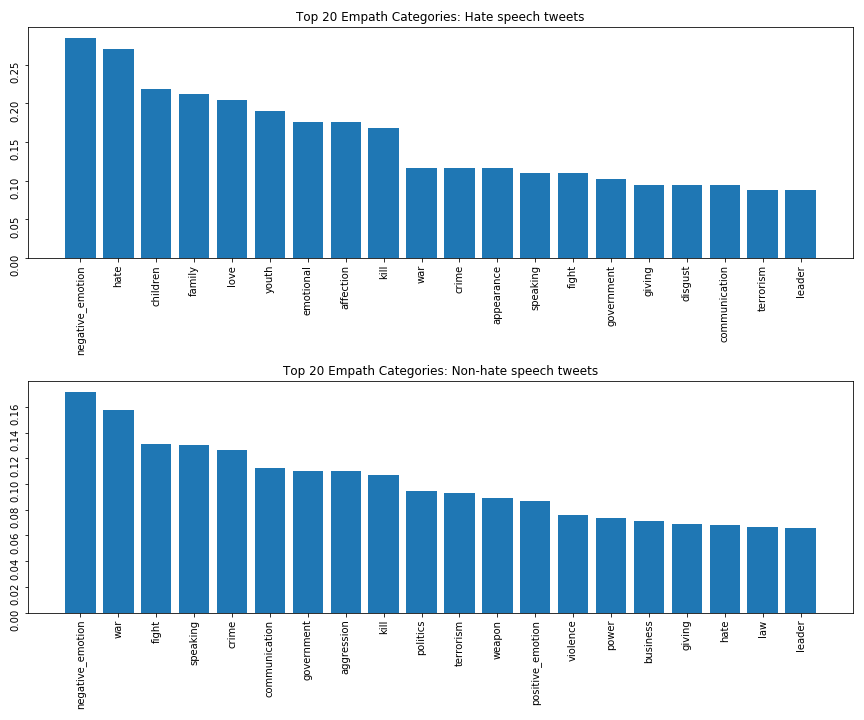
\includegraphics[width=5.0in]{liwc_topics} \label{fig:liwc_topics} \hfil 
\caption{Empath categories in the hate speech and non-hate speech tweets.}     
\end{figure*} 

\begin{figure*}[!t] 
    \centering 
    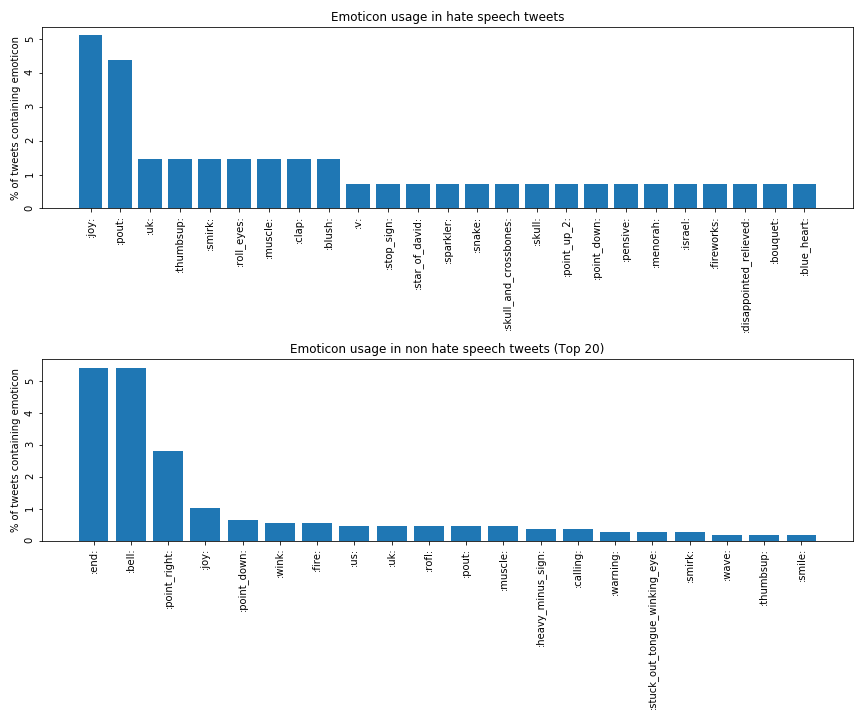
\includegraphics[width=5.0in]{emoticons} \label{fig:emoticon_usage} \hfil 
    \caption{Emoticon usage in the hate speech and non-hate speech tweets.}     
\end{figure*} 

\end{document}
    
    
